\documentclass[./main.tex]{subfiles}

\begin{document}

当我们第一次谈及函子时,得知这是一个用于映射的抽象概念。接着就是高级函子,让我们将某些类型视为在某些 contexts 中,保留 contexts
的同时还能应用普通函数在 contexts 中的值上。

本章我们开始学习单子 monads,它是一个增强版的高级函子,正如是一个高级函子是函子的增强版那样。

单子是高级函子的自然演进,可以这样考虑:如果有一个带 context 的值,\acode{m a},该如何将其应用至一个接受普通\acode{a}并返回一个
context 的函数?也就是说,如何应用一个类型为\acode{a -> m b}的函数至一个类型为\acode{m a}的值?概括一下就是想要一个这样的函数:

\begin{lstlisting}[language=Haskell]
  (>>=) :: (Monad m) => m a -> (a -> m b) -> m b
\end{lstlisting}

\textbf{当我们拥有一个漂亮的值以及一个接受普通值但返回漂亮值的函数,我们如何才能将漂亮值喂给这个函数?}这就是单子处理的主要问题。
这里用\acode{m a}而不是\acode{f a}是因为\acode{m}意为\acode{Monad},而单子就是支持\acode{>>=}操作的高级函子,此处的
\acode{>>=}函数读作\textit{绑定 bind}。

\subsection*{从处理\acode{Maybe}开始}

不出意外,\acode{Maybe}就是一个单子,让我看看它是如何以单子运作的。

\acode{Maybe a}代表一个类型\acode{a}的值处于有可能失败的 context 中。\acode{Just "dharma"}意为字符串\acode{"dharma"}
同时\acode{Nothing}代表着缺值,或者说如果将字符串作为计算的结果,那么\acode{Nothing}则代表计算失败了。

将\acode{Maybe}视为一个函子时,想要的是\acode{fmap}一个函数在其值,也就是\acode{Just}中的元素,否则保留\acode{Nothing}
状态,即内部没有任何元素。

\begin{lstlisting}[language=Haskell]
  ghci> fmap (++"!") (Just "wisdom")
  Just "wisdom!"
  ghci> fmap (++"!") Nothing
  Nothing
\end{lstlisting}

将\acode{Maybe}视为一个高级函子时,applicatives 同样包装了函数。使用\acode{<*>}应用一个函数在\acode{Maybe}内的值,
它们都必须是包在\acode{Just}来代表值存在,否则返回\acode{Nothing}。

\begin{lstlisting}[language=Haskell]
  ghci> Just (+3) <*> Just 3
  Just 6
  ghci> Nothing <*> Just "greed"
  Nothing
  ghci> Just ord <*> Nothing
  Nothing
\end{lstlisting}

当我们使用 applicative 风格让普通函数作用在\acode{Maybe}值时,所有的值都需要时\acode{Just}值,否则返回\acode{Nothing}!

\begin{lstlisting}[language=Haskell]
  ghci> max <$> Just 3 <*> Just 6
  Just 6
  ghci> max <$> Just 3 <*> Nothing
  Nothing
\end{lstlisting}

现在让我们想想该如何使用\acode{>>=}在\acode{Maybe}上。正如我们所说的,\acode{>>=}接受一个 monadic 值以及一个接受普通值并
返回一个 monadic 值的函数。

\acode{>>=}将接受一个\acode{Maybe a}值以及一个类型\acode{a -> Maybe a}的函数,以某种方式应用该函数至\acode{Maybe a}。
假设我们有一个函数\acode{\\x -> Just (x+1)}。它接受一个值,加\acode{1}并将其包装在一个\acode{Just}内。

\begin{lstlisting}[language=Haskell]
  ghci> (\x -> Just (x+1)) 1
  Just 2
  ghci> (\x -> Just (x+1)) 100
  Just 101
\end{lstlisting}

现在的问题是如何将一个\acode{Maybe}值喂给该函数?如果思考了\acode{Maybe}是如何作为一个高级函子的,那么该问题的答案就很简单了。
如果拿到一个\acode{Just},就把包在\acode{Just}内的值喂给函数;如果拿到一个\acode{Nothing}则返回\acode{Nothing}。

现在我们不调用\acode{>>=}而是调用\acode{applyMaybe},那么它接受一个\acode{Maybe a}以及一个返回\acode{Maybe b}的函数,
并将该函数应用至\acode{Maybe a}:

\begin{lstlisting}[language=Haskell]
  applyMaybe :: Maybe a -> (a -> Maybe b) -> Maybe b
  applyMaybe Nothing f  = Nothing
  applyMaybe (Just x) f = f x
\end{lstlisting}

现在让我们试试:

\begin{lstlisting}[language=Haskell]
  ghci> Just 3 `applyMaybe` \x -> Just (x+1)
  Just 4
  ghci> Just "smile" `applyMaybe` \x -> Just (x ++ " :)")
  Just "smile :)"
  ghci> Nothing `applyMaybe` \x -> Just (x+1)
  Nothing
  ghci> Nothing `applyMaybe` \x -> Just (x ++ " :)")
  Nothing
\end{lstlisting}

上述例子中,可以看到当使用\acode{applyMaybe}于一个\acode{Just}值以及一个函数,该函数很容易的就被应用到了\acode{Just}
内的值;而但作用于一个\acode{Nothing},那么结果就是\acode{Nothing}。那么如果函数返回的是\acode{Nothing}?

\begin{lstlisting}[language=Haskell]
  ghci> Just 3 `applyMaybe` \x -> if x > 2 then Just x else Nothing
  Just 3
  ghci> Just 1 `applyMaybe` \x -> if x > 2 then Just x else Nothing
  Nothing
\end{lstlisting}

符合预期。如果左侧的 monadic 值是\acode{Nothing},那么整个结果就是\acode{Nothing};如果右侧函数返回的是\acode{Nothing},
结果还是\acode{Nothing}。这非常像是使用\acode{Maybe}作为高级函子时,过程中有任何一个\acode{Nothing}时,整个结果就会是
\acode{Nothing}。

你或许会问,这样有用么?看起来高级函子比单子更强,因为高级函子允许我们用一个普通函数应用至 contexts 中的值上。而单子可以这么做
是因为它们是升级版的高级函子,那肯定是可以做高级函子不能做的事情。

稍后我们再来讨论\acode{Maybe},现在让我们看看属于单子的那些 typeclass。

\subsection*{单子 typeclass}

正如函子拥有\acode{Functor} typeclass,高级函子拥有\acode{Applicative} typeclass,单子也有自己的 typeclass:
\acode{Monad}!

\begin{lstlisting}[language=Haskell]
  class Monad m where
    return :: a -> m a

    (>>=) :: m a -> (a -> m b) -> m b

    (>>) :: m a -> m b -> m b
    x >> y = x >>= \_ -> y

    fail :: String -> m a
    fail msg = error msg
\end{lstlisting}

首先从第一行开始,\acode{class Monad m where}。等等之前不是提到过单子是高级函子的演进吗?那么不应该有一个类约束像是
\acode{class (Applicative m) => Monad m where},也就是一个类型必须先是高级函子才能是单子么?的确要有,但是 Haskell
被创造的早期,人们没有想到高级函子适合被放进语言中,所以最后并没有这个限制。但的确每个单子都是高级函子,即使\acode{Monad}
并没有这么宣告。

\acode{Monad} typeclass 的第一个函数定义就是\acode{return}。它等同于\acode{pure},只不过名字不同,其类型为
\acode{(Monad m) => a -> m a}。接受一个值,将其放入最小默认 context 中。对于\acode{Maybe}而言,就是将值放入
\acode{Just}中。

接下来的是函数\acode{>>=},或绑定。它像是函数应用那样,只不过它接受的不是普通值而是一个 monadic 值(即具有 context 的值)
并把该值喂给一个接受普通值的函数,最后返回一个 monadic 值。

接下来就是函数\acode{>>},现在无需太多的关注因为它拥有一个默认实现,同时在构造\acode{Monad}实例时我们几乎永远不用考虑去实现它。

最后的函数就是\acode{Monad} typeclass 的\acode{fail}。我们永远不会显式的在代码中用到,而是会被 Haskell 用在处理语法错误。
目前不需要太在意\acode{fail}。

现在来看一下\acode{Maybe}的\acode{Monad}实例。

\begin{lstlisting}[language=Haskell]
  instance Monad Maybe where
    return x = Just x
    Nothing >>= f = Nothing
    Just x >>= f  = f x
    fail _ = Nothing
\end{lstlisting}

\acode{return}与\acode{pure}等价。

\acode{>>=}与\acode{applyMaybe}是一样的。当\acode{Maybe a}喂给我们函数时,我们保留 context,并在左值为\acode{Nothing}
时返回\acode{Nothing},左值为\acode{Just}时将\acode{f}应用至其内部值。

\begin{lstlisting}[language=Haskell]
  ghci> return "WHAT" :: Maybe String
  Just "WHAT"
  ghci> Just 9 >>= \x -> return (x*10)
  Just 90
  ghci> Nothing >>= \x -> return (x*10)
  Nothing
\end{lstlisting}

我们已经在\acode{Maybe}使用过\acode{pure}了,这里的\acode{return}就是\acode{pure}。

注意是如何把\acode{Just 9}喂给\acode{\\x -> return (x*10)}的。在函数中\acode{x}绑定到\acode{9}。它看起来不用模式匹配
就能从\acode{Maybe}中抽取值,且并没有丢失\acode{Maybe}的 context。

\subsection*{走钢丝}

现在我们知道了如何将一个\acode{Maybe a}值喂给\acode{a -> Maybe b}类型的函数。现在看看我们如何重复使用\acode{>>=}来处理多个
\acode{Maybe a}值。

...省略原文故事。

我们用一对整数来代表平衡杆的状态。第一个位置代表左侧的鸟的数量,第二个位置代表右侧的鸟的数量。

\begin{lstlisting}[language=Haskell]
  type Birds = Int
  type Pole = (Birds,Birds)
\end{lstlisting}

接下来定义两个函数,它们接受一个代表鸟的数量的数值以及分别放在杆子的左右侧。

\begin{lstlisting}[language=Haskell]
  landLeft :: Birds -> Pole -> Pole
  landLeft n (left,right) = (left + n,right)

  landRight :: Birds -> Pole -> Pole
  landRight n (left,right) = (left,right + n)
\end{lstlisting}

测试:

\begin{lstlisting}[language=Haskell]
  ghci> landLeft 2 (0,0)
  (2,0)
  ghci> landRight 1 (1,2)
  (1,3)
  ghci> landRight (-1) (1,2)
  (1,1)
\end{lstlisting}

鸟儿飞走只需要用负值表达即可。由于函数的输入与返回都是\acode{Pole}的缘故,我们可以串联\acode{landLeft}与\acode{landRight}:

\begin{lstlisting}[language=Haskell]
  ghci> landLeft 2 (landRight 1 (landLeft 1 (0,0)))
  (3,1)
\end{lstlisting}

如果编写这样的一个函数:

\begin{lstlisting}[language=Haskell]
  x -: f = f x
\end{lstlisting}

那么就可以先写参数,然后再是函数:

\begin{lstlisting}[language=Haskell]
  ghci> 100 -: (*3)
  300
  ghci> True -: not
  False
  ghci> (0,0) -: landLeft 2
  (2,0)
\end{lstlisting}

使用这样的方法我们可以用更加可读的方式来重复之前的表达:

\begin{lstlisting}[language=Haskell]
  ghci> (0,0) -: landLeft 1 -: landRight 1 -: landLeft 2
  (3,1)
\end{lstlisting}

那么如果一次性飞入 10 只鸟儿呢?

\begin{lstlisting}[language=Haskell]
  ghci> landLeft 10 (0,3)
  (10,3)
\end{lstlisting}

平衡杆会失去平衡(超过 4 只鸟)!这是显而易见的,但是如果在一系列的操作当中:

\begin{lstlisting}[language=Haskell]
  ghci> (0,0) -: landLeft 1 -: landRight 4 -: landLeft (-1) -: landRight (-2)
  (0,2)
\end{lstlisting}

这看起来没问题,但是实际上中间有一刻是右侧有 4 只鸟,而左侧没有鸟!修复这个问题,我们需重审\acode{landLeft}与\acode{landRight}
函数。这些函数是需要返回失败的。这就是使用\acode{Maybe}的绝佳时刻!

\begin{lstlisting}[language=Haskell]
  landLeft :: Birds -> Pole -> Maybe Pole
  landLeft n (left, right)
    | abs ((left + n) - right) < 4 = Just (left + n, right)
    | otherwise = Nothing

  landRight :: Birds -> Pole -> Maybe Pole
  landRight n (left, right)
    | abs (left - (right + n)) < 4 = Just (left, right + n)
    | otherwise = Nothing
\end{lstlisting}

测试:

\begin{lstlisting}[language=Haskell]
  ghci> landLeft 2 (0,0)
  Just (2,0)
  ghci> landLeft 10 (0,3)
  Nothing
\end{lstlisting}

现在我们需要一种方法,接受一个\acode{Maybe Pole},将其喂给接受\acode{Pole}并返回\acode{Maybe Pole}的函数。幸运的是,我们
拥有\acode{>>=}:

\begin{lstlisting}[language=Haskell]
  ghci> landRight 1 (0,0) >>= landLeft 2
  Just (2,1)
\end{lstlisting}

注意,\acode{landLeft 2}的类型是\acode{Pole -> Maybe Pole}。我们无法将\acode{landRight 1 (0,0)}的\acode{Maybe Pole}
结果喂给它,因此使用了\acode{>>=}来将带有 context 的值给到了\acode{landLeft 2}。\acode{>>=}确实允许我们将\acode{Maybe}
值视为一个带有 context 的值,因为如果将一个\acode{Nothing}喂给\acode{landLeft 2},那么结果就是\acode{Nothing}且失败被
传递下去:

\begin{lstlisting}[language=Haskell]
  ghci> Nothing >>= landLeft 2
  Nothing
\end{lstlisting}

测试一系列的操作:

\begin{lstlisting}[language=Haskell]
  ghci> return (0,0) >>= landRight 2 >>= landLeft 2 >>= landRight 2
  Just (2,4)
\end{lstlisting}

开始时通过\acode{return}将一个 pole 包装进一个\acode{Just}。

稍早之前的一系列操作:

\begin{lstlisting}[language=Haskell]
  ghci> return (0,0) >>= landLeft 1 >>= landRight 4 >>= landLeft (-1) >>= landRight (-2)
  Nothing
\end{lstlisting}

符合预期,最后的情形代表了失败的情况。

如果只把\acode{Maybe}当做高级函子使用的话是没有办法达到我们想要的效果。因为高级函子并不允许 applicative 值之间有弹性的交互。
它们最多就是让我们可以用 applicative 风格来传递参数至函数。applicative 操作符拿到它们的结果并用 applicative 的方式喂给
另一个函数,最后将最终的 applicative 值放在一起。这里面每一步之间并没有多少操作空间。而我们的这个例子需要的是每一步都依赖前一步的
结果。

我们也可以写一个\acode{banana}函数必定返回失败:

\begin{lstlisting}[language=Haskell]
  banana :: Pole -> Maybe Pole
  banana _ = Nothing
\end{lstlisting}

将该函数置于整个过程中,不管前面的状态如何,都会产生失败:

\begin{lstlisting}[language=Haskell]
  ghci> return (0,0) >>= landLeft 1 >>= banana >>= landRight 1
  Nothing
\end{lstlisting}

\acode{Just (1,0)}被喂给\acode{banana}产生\acode{Nothing}之后所有的结果便是\acode{Nothing}了。

除开构建一个忽略输入并返回一个预先设定好的 monadic 值,还可以使用\acode{>>}函数,其默认实现如下:

\begin{lstlisting}[language=Haskell]
  (>>) :: (Monad m) => m a -> m b -> m b
  m >> n = m >>= \_ -> n
\end{lstlisting}

一般而言,碰到一个完全忽略前面状态的函数,它就只会返回它想返回的值。然而碰到单子时,它们的 context 还是必须要被考虑到的。看一下
\acode{>>}串联\acode{Maybe}的情况。

\begin{lstlisting}[language=Haskell]
  ghci> Nothing >> Just 3
  Nothing
  ghci> Just 3 >> Just 4
  Just 4
  ghci> Just 3 >> Nothing
  Nothing
\end{lstlisting}

如果把\acode{>>}换成\acode{>>= \\_ ->},就很容易理解了。

将\acode{banana}改用\acode{>>}与\acode{Nothing}来表达:

\begin{lstlisting}[language=Haskell]
  ghci> return (0,0) >>= landLeft 1 >> Nothing >>= landRight 1
  Nothing
\end{lstlisting}

注意\acode{Maybe}对\acode{>>=}的实现,它其实就是在遇到\acode{Nothing}时返回\acode{Nothing},遇到\acode{Just}值时
继续用\acode{Just}传值。

\subsection*{do 表示法}

Haskell 中的单子非常的有用,它们得到了属于自己的特殊语法,即\acode{do}表示法。我们已经学习到了\acode{do}标记法用作 I/O,
同时将若干 I/O actions 粘合成为一个。实际上\acode{do}表示法不仅仅作用于\acode{IO},而是可以用于任意单子。其原则仍然不变:
顺序的粘合其他的 monadic 值。现在让我们看看\acode{do}表示法是如何工作的,以及为什么这么有用。

考虑以下 monadic 应用的例子:

\begin{lstlisting}[language=Haskell]
  ghci> Just 3 >>= (\x -> Just (show x ++ "!"))
  Just "3!"
\end{lstlisting}

那么如果还有另一个\acode{>>=}在函数内呢?

\begin{lstlisting}[language=Haskell]
  ghci> Just 3 >>= (\x -> Just "!" >>= (\y -> Just (show x ++ y)))
  Just "3!"
\end{lstlisting}

一个嵌套的\acode{>>=}!在最外层的 lambda 函数,将\acode{Just "!"}喂给 lambda \acode{\\y -> Just (show x ++ y)}。
在内部的 lambda,\acode{y}变成\acode{"!"}。\acode{x}仍然是\acode{3}因为是从外层的 lambda 取值的。这些行为让我们想到了
下列式子:

\begin{lstlisting}[language=Haskell]
  ghci> let x = 3; y = "!" in show x ++ y
  "3!"
\end{lstlisting}

差别在于前者的值是 monadic,带有可能失败的 context。我们可以把其中任何一步替换成失败的状态:

\begin{lstlisting}[language=Haskell]
  ghci> Nothing >>= (\x -> Just "!" >>= (\y -> Just (show x ++ y)))
  Nothing
  ghci> Just 3 >>= (\x -> Nothing >>= (\y -> Just (show x ++ y)))
  Nothing
  ghci> Just 3 >>= (\x -> Just "!" >>= (\y -> Nothing))
  Nothing
\end{lstlisting}

为了解释的更清楚,我们来编写一个自己的\acode{Maybe}脚本:

\begin{lstlisting}[language=Haskell]
  foo :: Maybe String
  foo = Just 3 >>= (\x -> Just "!" >>= (\y -> Just (show x ++ y)))
\end{lstlisting}

为了避免这些麻烦的 lambda,Haskell 允许我们使用\acode{do}表示法:

\begin{lstlisting}[language=Haskell]
  foo :: Maybe String
  foo = do
    x <- Just 3
    y <- Just "!"
    Just (show x ++ y)
\end{lstlisting}

看起来好像是不必每一步都去检查\acode{Maybe}值是\acode{Just}或\acode{Nothing}。如果任意步骤取出了\acode{Nothing},
那么整个\acode{do}的结果就会是\acode{Nothing}。我们把所有责任都交给\acode{>>=},它来处理所有的\acode{context}问题。
这里的\acode{do}表示法就是另一种语法的形式来串联所有的 monadic 值。

在\acode{do}表达式中,每一行都是一个 monadic 值。想要获取结果,需要\acode{<-}。如果有一个\acode{Maybe String},
同时我们通过\acode{<-}绑定它到一个变量上,那么该变量将变为一个\acode{String},就像是我们使用\acode{>>=}将 monadic
值喂给 lambdas 那样。\acode{do}表达式中,最后一个 monadic 值,例如这里的\acode{Just (show x ++ y)},不可以将它
绑定至一个结果,因为这样的写法转换成\acode{>>=}的结果时不合理。它必须是所有 monadic 值粘合后最终的结果,因此需要考虑前面
所有可能失败的情景。

例如以下:

\begin{lstlisting}[language=Haskell]
  ghci> Just 9 >>= (\x -> Just (x > 8))
  Just True
\end{lstlisting}

因为\acode{>>=}的左参是一个\acode{Just}值,lambda 被应用至\acode{9},同时返回是一个\acode{Just True}。如果将上述
重写为\acode{do}表示法,可得:

\begin{lstlisting}[language=Haskell]
  marySue :: Maybe Bool
  marySue = do
      x <- Just 9
      Just (x > 8)
\end{lstlisting}

比较这两种写法,很容易看出来为什么整个 monadic 值的结果会是在\acode{do}表示法中最后一个,因为它串联了前面所有的结果。

用\acode{do}表示法来改写 routine 函数:

\begin{lstlisting}[language=Haskell]
  routine :: Maybe Pole
  routine = do
    start <- return (0,0)
    first <- landLeft 2 start
    second <- landRight 2 first
    landLeft 1 second
\end{lstlisting}

测试:

\begin{lstlisting}[language=Haskell]
  ghci> routine
  Just (3,2)
\end{lstlisting}

中间插入香蕉皮:

\begin{lstlisting}[language=Haskell]
  routine :: Maybe Pole
  routine = do
      start <- return (0,0)
      first <- landLeft 2 start
      Nothing
      second <- landRight 2 first
      landLeft 1 second
\end{lstlisting}

在\acode{do}表示法中没有通过\acode{<-}绑定 monadic 值时,就像是将\acode{>>}放在 monadic 值之后,即忽略计算的结果。
我们只是要让它们有序,而不是要它们的结果,而且这比写\acode{_ <- Nothing}要好看。

何时使用\acode{do}表示法或是\acode{>>=}取决于你。

在\acode{do}表示法中,我们还可以用模式匹配来绑定 monadic 值,就好像我们在\acode{let}表达式以及函数参数那样:

\begin{lstlisting}[language=Haskell]
  justH :: Maybe Char
  justH = do
    (x : xs) <- Just "hello"
    return x
\end{lstlisting}

如果这个模式匹配失败了呢?函数中的模式匹配失败后会去匹配下一个模式,如果所有的模式都匹配不上,那么错误将被抛出,然后程序就
挂掉了。另一方面,如果在\acode{let}中进行模式匹配失败会直接抛出错误。毕竟在\acode{let}表达式的情况下没有失败就跳至下一个
选项的设计。至于在\acode{do}表示法中模式匹配失败时,就会调用\acode{fail}函数。它是\acode{Monad} typeclass 中的一部分,
它运行在现在的 context 下失败时不会挂掉程序。它的默认实现如下:

\begin{lstlisting}[language=Haskell]
  fail :: (Monad m) => String -> m a
  fail msg = error msg
\end{lstlisting}

默认情况下确实是让程序崩溃,不过一些单子(例如\acode{Maybe})表示可能失败的 context 时,通常会实现自己的失败函数。例如
\acode{Maybe}的实现如下:

\begin{lstlisting}[language=Haskell]
  fail _ = Nothing
\end{lstlisting}

它忽视所有错误并创造一个\acode{Nothing}。

\begin{lstlisting}[language=Haskell]
  justH :: Maybe Char
  justH = do
    (x : _) <- Just "hello";
    return x
\end{lstlisting}

这里模式匹配失败,产生的影响等同于一个\acode{Nothing}。测试:

\begin{lstlisting}[language=Haskell]
  ghci> wopwop
  Nothing
\end{lstlisting}

这样模式匹配的失败只会限制在单子的 context 中,而不会让程序崩溃,这样的处理方式好很多。

\subsection*{列表单子}

目前为止我们学习了\acode{Maybe}是如何被视为可能失败的 context,也学习了如何用\acode{>>=}来把这些可能失败的值传给函数。
这一小节中,我们开始学习如何用列表的 monadic 性质来写非确定性 non-deterministic 的程序。

把列表当做高级函子有如下特性:

\begin{lstlisting}[language=Haskell]
  ghci> (*) <$> [1,2,3] <*> [10,100,1000]
  [10,100,1000,20,200,2000,30,300,3000]
\end{lstlisting}

所有可能的组合相乘。

这个非确定性的 context 可以很漂亮的转换为单子。列表的\acode{Monad}实例如下:

\begin{lstlisting}[language=Haskell]
  instance Monad [] where
  return x = [x]
  xs >>= f = concat (map f xs)
  fail _ = []
\end{lstlisting}

\acode{return}即\acode{pure},不多赘述。

\acode{>>=}意为接受一个带有 context 的值(一个 monadic 值),将其喂给一个接受普通值的函数并返回一个带有 context 的值。
尝试一下将一个非确定性值喂给一个函数:

\begin{lstlisting}[language=Haskell]
  ghci> [3,4,5] >>= \x -> [x,-x]
  [3,-3,4,-4,5,-5]
\end{lstlisting}

在对\acode{Maybe}使用\acode{>>=}时,monadic 值喂给函数时考虑到了可能失败的 context。而列表的\acode{>>=}则考虑到了
非确定性。\acode{[3,4,5]}是一个非确定性的值,将它喂给一个返回非确定性值的函数,那么结果也会是非确定性的。该函数接受一个
数值并生产两个结果:一个负数,一个正数。因此当使用\acode{>>=}将这个列表喂给函数,每个列表中的数值保留了原有的符号,又新增了
相反符号的值。

为了了解这是如何做到的,我们仅需跟着实现。首先起始的是列表\acode{[3,4,5]},接着将 lambda 应用在它们上,得到:

\begin{lstlisting}[language=Haskell]
  [[3,-3],[4,-4],[5,-5]]
\end{lstlisting}

lambda 应用在了列表中的每个元素上,最后打平列表,这样就应用了一个非确定性的函数至一个非确定性的值了!

非确定性也有考虑到失败的可能。\acode{[]}其实就等价于\acode{Nothing},因为它没有结果。所以失败等同于返回一个空列表。

\begin{lstlisting}[language=Haskell]
  ghci> [] >>= \x -> ["bad","mad","rad"]
  []
  ghci> [1,2,3] >>= \x -> []
  []
\end{lstlisting}

和\acode{Maybe}一样,我们可以用\acode{>>=}把它们串起来:

\begin{lstlisting}[language=Haskell]
  ghci> [1,2] >>= \n -> ['a','b'] >>= \ch -> return (n,ch)
  [(1,'a'),(1,'b'),(2,'a'),(2,'b')]
\end{lstlisting}

\begin{figure}[h]
  \centering
  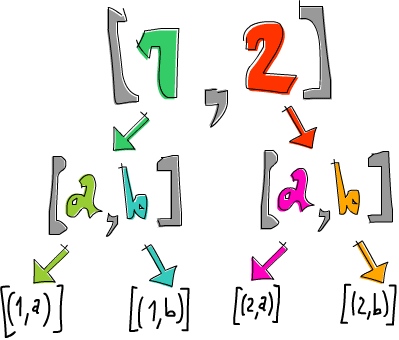
\includegraphics[width=0.6\textwidth]{\subfix{./images/concatmap.png}}
\end{figure}

列表\acode{[1,2]}绑定至\acode{n},\acode{['a','b']}绑定至\acode{ch}。接着使用\acode{return (n,ch)}(或是
\acode{[(n,ch)]}),意为将一对\acode{n,ch}并将其放入默认最小 context 中。可以这么理解:对于\acode{[1,2]}中的
每个元素而言,经历\acode{['a','b']}中每个元素,并生产一对元组。

一般而言,\acode{return}接受一个值并将其放入最小默认 context 中,它是不会多做额外的事情,仅仅只是用于展出结果。

\begin{anote}
  在处理非确定性值的时候,可以把列表中的每个元素想象成计算路线中的一个分支。
\end{anote}

将之前的表达式用\acode{do}重写:

\begin{lstlisting}[language=Haskell]
  listOfTuples :: [(Int, Char)]
  listOfTuples = do
    n <- [1, 2]
    ch <- ['a', 'b']
    return (n, ch)
\end{lstlisting}

这样写可以更清楚的知道\acode{n}走过\acode{[1,2]}中的每个值,而\acode{ch}则走过\acode{['a','b']}中的每个值。
正如\acode{Maybe}那样,从 monadic 值中取出普通值再喂给函数。\acode{>>=}会帮我们处理好一切 context 相关的问题,
不同之处在于列表的 context 指的是非确定性。

使用\acode{do}表示法很想我们之前做的:

\begin{lstlisting}[language=Haskell]
  ghci> [ (n,ch) | n <- [1,2], ch <- ['a','b'] ]
  [(1,'a'),(1,'b'),(2,'a'),(2,'b')]
\end{lstlisting}

正是列表表达式!在之前的\acode{do}表达式的例子中,\acode{n}走过\acode{[1,2]}的每个元素,\acode{ch}走过
\acode{['a','b']}的每个元素,接着把\acode{(n,ch)}放进一个 context 中。这跟列表表达式的目的一样,只是列表表达式
不需要在最后用\acode{return}来得到\acode{(n,ch)}结果。

实际上,列表表达式是一个语法糖。无论是列表表达式还是\acode{do}表示法,都会转换成使用\acode{>>=}来做非确定性特征的计算。

列表表达式允许我们过滤输出。例如仅收集含有数字\acode{7}的数字:

\begin{lstlisting}[language=Haskell]
  ghci> [ x | x <- [1..50], '7' `elem` show x ]
  [7,17,27,37,47]
\end{lstlisting}

我们将\acode{show}应用至\acode{x}上使数值变为字符串再查看字符\acode{'7'}是否存在在字符串中。为了知道筛选列表表达式
是如何转换成列表单子的,我们需要检查\acode{guard}函数以及\acode{MonadPlus} typeclass。该 typeclass 用于表达同时
可以表现为幺半群的单子,以下是其定义:

\begin{lstlisting}[language=Haskell]
  class Monad m => MonadPlus m where
    mzero :: m a
    mplus :: m a -> m a -> m a
\end{lstlisting}

\acode{mzero}是\acode{Monoid} typeclass 中\acode{mempty}的同义词,\acode{mplus}则关联\acode{maapend}。
列表既是幺半群又是单子,因此可以实现\acode{MonadPlus}这个 typeclass:

\begin{lstlisting}[language=Haskell]
  instance MonadPlus [] where
    mzero = []
    mplus = (++)
\end{lstlisting}

对于列表而言,\acode{mzero}代表一个非确定性计算且没有任何结果 -- 一个失败的计算,\acode{mplus}将两个非确定性的值
结合成一个。\acode{guard}函数定义如下:

\begin{lstlisting}[language=Haskell]
  guard :: (MonadPlus m) => Bool -> m ()
  guard True = return ()
  guard False = mzero
\end{lstlisting}

它接受一个布尔值,如果为\acode{True},则接受一个\acode{()}并将其置入最小默认 context 中代表成功;否则创建一个失败的
monadic 值。

\begin{lstlisting}[language=Haskell]
  ghci> guard (5 > 2) :: Maybe ()
  Just ()
  ghci> guard (1 > 2) :: Maybe ()
  Nothing
  ghci> guard (5 > 2) :: [()]
  [()]
  ghci> guard (1 > 2) :: [()]
  []
\end{lstlisting}

看起来很有趣,不过如何有用呢?在列表单子中,我们用它来过滤非确定性计算。

\begin{lstlisting}[language=Haskell]
  ghci> [1..50] >>= (\x -> guard ('7' `elem` show x) >> return x)
  [7,17,27,37,47]
\end{lstlisting}

这里的结果与之前的列表表达式是一致的。那么\acode{guard}是如何工作的呢?让我们看看\acode{guard}函数是如何与\acode{>>}
关联的:

\begin{lstlisting}[language=Haskell]
  ghci> guard (5 > 2) >> return "cool" :: [String]
  ["cool"]
  ghci> guard (1 > 2) >> return "cool" :: [String]
  []
\end{lstlisting}

如果\acode{guard}成功,得到一个空的元组,接着用\acode{>>}来忽略空的元组,得到不同的结果;反之,\acode{return}失败。
这是因为用\acode{>>=}把空的列表喂给函数总是返回空的列表。\acode{guard}大致的意思就是:如果一个布尔值为\acode{False}
那么久产生一个失败的状态,反之返回一个\acode{()}。如此计算可以继续进行。

用\acode{do}改写之前的例子:

\begin{lstlisting}[language=Haskell]
  sevensOnly :: [Int]
  sevensOnly = do
    x <- [1 .. 50]
    guard ('7' `elem` show x)
    return x
\end{lstlisting}

这里不写最后一行的\acode{return x},整个列表就会是包含一堆空元组的列表。

上述例子写成列表表达式就是这样:

\begin{lstlisting}[language=Haskell]
  ghci> [ x | x <- [1..50], '7' `elem` show x ]
  [7,17,27,37,47]
\end{lstlisting}

因此列表表达式的过滤基本上跟\acode{guard}是一致的。

\subsubsection*{一个骑士任务}

这里有一个用非确定性解决的问题。假设有一个棋盘以及一个骑士棋子,我们想要知道骑士是否可以在三步之内移动到想要的位置。
我们只需要一对数值来表示骑士在棋盘上的位置。第一个数值代表棋盘行数,第二个代表列数。

\newpage
\begin{figure}[h]
  \centering
  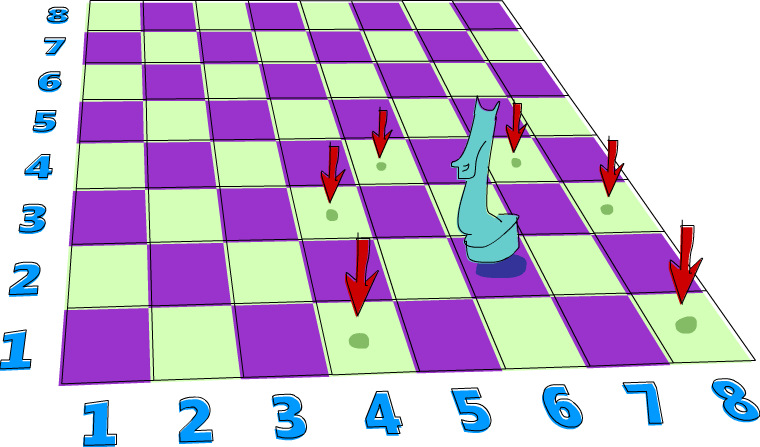
\includegraphics[width=0.8\textwidth]{\subfix{./images/chess.png}}
\end{figure}

用一个类型来模拟骑士所处棋盘的位置:

\begin{lstlisting}[language=Haskell]
  type KnightPos = (Int, Int)
\end{lstlisting}

假设起始点\acode{(6,2)},那么能用三步到\acode{(6,1)}么?下一步的最优解是什么?不如全部一起考虑!要好好利用所谓的
非确定性。所有我们不是只选择一步,而是选择全部。首先写一个函数返回所有可能的下一步:

\begin{lstlisting}[language=Haskell]
  moveKnight :: KnightPos -> [KnightPos]
  moveKnight (c, r) = do
    (c', r') <-
      [ (c + 2, r - 1),
        (c + 2, r + 1),
        (c - 2, r - 1),
        (c - 2, r + 1),
        (c + 1, r - 2),
        (c + 1, r + 2),
        (c - 1, r - 2),
        (c - 1, r + 2)
        ]
    guard (c' `elem` [1 .. 8] && r' `elem` [1 .. 8])
    return (c', r')
\end{lstlisting}

骑士的移动为日字形(参考象棋中的马)即横一竖二或者横二竖一。\acode{(c',r')}走过列表中的每个元素,\acode{guard}用于
保证移动后停留在棋盘上,否则产生一个空的列表代表失败,这样\acode{return (c',r')}就不会执行。

如果不用列表单子写,那么也可以用\acode{filter}来实现:

\begin{lstlisting}[language=Haskell]
  moveKnight :: KnightPos -> [KnightPos]
  moveKnight (c, r) =
    filter
      onBoard
      [ (c + 2, r - 1),
        (c + 2, r + 1),
        (c - 2, r - 1),
        (c - 2, r + 1),
        (c + 1, r - 2),
        (c + 1, r + 2),
        (c - 1, r - 2),
        (c - 1, r + 2)
      ]
    where
      onBoard (c, r) = c `elem` [1 .. 8] && r `elem` [1 .. 8]
\end{lstlisting}

测试:

\begin{lstlisting}[language=Haskell]
  ghci> moveKnight (6,2)
  [(8,1),(8,3),(4,1),(4,3),(7,4),(5,4)]
  ghci> moveKnight (8,1)
  [(6,2),(7,3)]
\end{lstlisting}

接下来就是\acode{in3}函数,接受一个起始位置,每一步都是一个非确定性的位置,然后用\acode{>>=}喂给\acode{moveKnight}:

\begin{lstlisting}[language=Haskell]
  in3 :: KnightPos -> [KnightPos]
  in3 start = do
    first <- moveKnight start
    second <- moveKnight first
    moveKnight second
\end{lstlisting}

也可以不使用\acode{do}:

\begin{lstlisting}[language=Haskell]
  in3 start = return start >>= moveKnight >>= moveKnight >>= moveKnight
\end{lstlisting}

接下来就是接受两个位置并测试是否可以三步内移动到指定位置的函数:

\begin{lstlisting}[language=Haskell]
  canReachIn3 :: KnightPos -> KnightPos -> Bool
  canReachIn3 start end = end `elem` in3 start
\end{lstlisting}

测试:

\begin{lstlisting}[language=Haskell]
  ghci> (6,2) `canReachIn3` (6,1)
  True
  ghci> (6,2) `canReachIn3` (7,3)
  False
\end{lstlisting}

\subsection*{单子定律}

% TODO

% \begin{lstlisting}[language=Haskell]

% \end{lstlisting}

\end{document}
